% --- HEADER ---
\noindent\hspace*{160pt}\begin{minipage}{344pt}
  {\small\textbf{\textsf{\color{stewartblue}MỤC 2.8}}\quad \textsf{Đạo hàm dưới dạng một hàm số}\hfill \textbf{\textsf{161}}}
\end{minipage}
\vspace{0.8em}

% --- MAIN TEXT (CỘT NỘI DUNG CHÍNH LỆCH PHẢI) ---
\noindent\hspace*{160pt}\begin{minipage}{344pt}
  Chúng ta cũng có thể diễn giải đạo hàm cấp ba về mặt vật lý trong trường hợp hàm số là hàm vị trí $s = s(t)$ của một vật chuyển động trên một đường thẳng. Vì $s''' = (s'')' = a'$, nên đạo hàm cấp ba của hàm vị trí chính là đạo hàm của hàm gia tốc và được gọi là \textbf{độ giật (jerk)}:
  \[
    j = \frac{da}{dt} = \frac{d^3s}{dt^3}
  \]
  Do đó độ giật $j$ là tốc độ thay đổi của gia tốc. Nó được đặt tên rất xác đáng vì một độ giật lớn đồng nghĩa với sự thay đổi đột ngột của gia tốc, gây ra chuyển động giật cục.

  Quá trình lấy đạo hàm có thể được tiếp tục. Đạo hàm cấp bốn $f''''$ thường được ký hiệu là $f^{(4)}$. Nói chung, đạo hàm cấp $n$ của $f$ được ký hiệu là $f^{(n)}$ và thu được từ $f$ bằng cách lấy đạo hàm $n$ lần. Nếu $y = f(x)$, ta viết
  \[
    y^{(n)} = f^{(n)}(x) = \frac{d^ny}{dx^n}
  \]

  \textbf{\color{stewartblue}VÍ DỤ 7}\quad Nếu $f(x) = x^3 - x$, hãy tìm $f'''(x)$ và $f^{(4)}(x)$.

  \textbf{\color{stewartblue}LỜI GIẢI}\quad Trong Ví dụ 6 chúng ta đã tìm được $f''(x) = 6x$. Đồ thị của đạo hàm cấp hai có phương trình $y = 6x$ và do đó nó là một đường thẳng có hệ số góc bằng 6. Vì đạo hàm $f'''(x)$ là hệ số góc của $f''(x)$, ta có
  \[
    f'''(x) = 6
  \]
  với mọi giá trị của $x$. Do đó $f'''$ là một hàm hằng và đồ thị của nó là một đường thẳng nằm ngang. Vì vậy, với mọi giá trị của $x$,
  \[
    f^{(4)}(x) = 0 \tag*{\color{stewartblue}$\blacksquare$}
  \]

  Chúng ta đã thấy rằng một ứng dụng của đạo hàm cấp hai và cấp ba xuất hiện trong việc phân tích chuyển động của các vật thể sử dụng gia tốc và độ giật. Chúng ta sẽ nghiên cứu một ứng dụng khác của đạo hàm cấp hai trong Mục 4.3, nơi chúng ta chỉ ra hiểu biết về $f''$ cho ta thông tin về hình dạng của đồ thị $f$ như thế nào. Trong Chương 11, chúng ta sẽ thấy đạo hàm cấp hai và các đạo hàm cấp cao hơn cho phép chúng ta biểu diễn các hàm số dưới dạng tổng của các chuỗi vô hạn.
\end{minipage}

\vspace{1.5em}

% --- EXERCISES BANNER (TRẢI RỘNG TOÀN TRANG) ---
\noindent
\begin{minipage}[c]{115pt}
  \color{stewartblue!60}
  \hrule height 0.6pt\vspace{2pt}
  \hrule height 0.6pt\vspace{2pt}
  \hrule height 0.6pt\vspace{2pt}
  \hrule height 0.6pt
\end{minipage}%
\hspace{8pt}%
\begin{minipage}[c]{120pt}
  \centering
  {\Large\bfseries\color{stewartblue} 2.8}\;
  {\color{stewartblue}\vrule width 1.2pt height 13pt depth 2pt}\;
  {\Large\bfseries Bài tập}
\end{minipage}%
\hspace{8pt}%
\begin{minipage}[c]{253pt}
  \color{stewartblue!60}
  \hrule height 0.6pt\vspace{2pt}
  \hrule height 0.6pt\vspace{2pt}
  \hrule height 0.6pt\vspace{2pt}
  \hrule height 0.6pt
\end{minipage}

\vspace{1.2em}

% --- EXERCISES 2-COLUMN LAYOUT ---
\noindent
\begin{minipage}[t]{242pt}
  \textbf{\color{stewartblue}1--2}\enskip Sử dụng đồ thị đã cho để ước lượng giá trị của mỗi đạo hàm. Sau đó phác thảo đồ thị của $f'$.

  \vspace{0.8em}
  \textbf{1.}\enskip
  \begin{tabular}[t]{@{}llll@{}}
    (a) $f'(0)$ & (b) $f'(1)$ & (c) $f'(2)$ & (d) $f'(3)$ \\[4pt]
    (e) $f'(4)$ & (f) $f'(5)$ & (g) $f'(6)$ & (h) $f'(7)$
  \end{tabular}

  \vspace{0.8em}
  \centering
  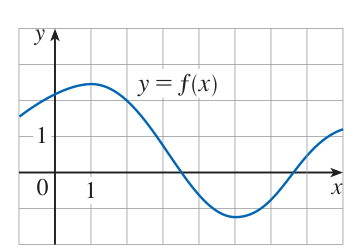
\includegraphics[width=0.74\linewidth]{images/p0196_fig1.png}
\end{minipage}%
\hfill%
\begin{minipage}[t]{242pt}
  \textbf{2.}\enskip
  \begin{tabular}[t]{@{}lll@{}}
    (a) $f'(-3)$ & (b) $f'(-2)$ & (c) $f'(-1)$ \\[4pt]
    (d) $f'(0)$  & (e) $f'(1)$  & (f) $f'(2)$  \\[4pt]
    (g) $f'(3)$  &              &
  \end{tabular}

  \vspace{1.2em}
  \centering
  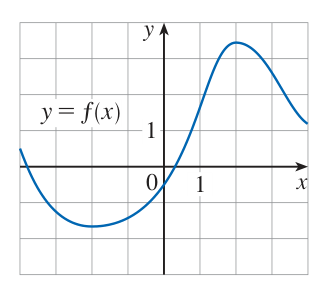
\includegraphics[width=0.64\linewidth]{images/p0196_fig2.png}
\end{minipage}

\vspace*{\fill}

% --- COPYRIGHT FOOTER ---
\noindent\rule{\textwidth}{0.4pt}
\vspace{1pt}
\centerline{\fontsize{6}{7.5}\selectfont\color{gray} Copyright 2021 Cengage Learning. All Rights Reserved. May not be copied, scanned, or duplicated, in whole or in part. WCN 02-200-203}
\centerline{\fontsize{5.5}{7}\selectfont\color{gray} Copyright 2021 Cengage Learning. All Rights Reserved. May not be copied, scanned, or duplicated, in whole or in part. Due to electronic rights, some third party content may be suppressed from the eBook and/or eChapter(s).}
\centerline{\fontsize{5.5}{7}\selectfont\color{gray} Editorial review has deemed that any suppressed content does not materially affect the overall learning experience. Cengage Learning reserves the right to remove additional content at any time if subsequent rights restrictions require it.}
